\section{Conclusions}
\label{sec:conclusions}

Overall findings indicate that AMD’s \gls{SMU} (via the \texttt{ryzen\_smu}
kernel driver) and the \gls{RAPL} interface provide different numerical
estimates of energy consumption for identical workloads and have no proven
correlation or similarity.

While this does not preclude the existence of more subtle "trends" and
similarities, such effects were not detectable within the scope and time
constraints of the present work.

Large discrepancies in absolute values can be explained by both imperfections
in the \emph{Ryzen Plugin} implementation (values interpretation and/or conversion
errors, numerical types conversion issues, inappropriate/imperfect method for
integrating power into energy, etc.) and lack of official documentation regarding
the access to these values.

In conclusion, the  AMD telemetry access interfaces may offer advantages over 
alternatives in several important respects, provided the deficiencies in the
methodology and implementations presented in this paper are addressed.
Potential areas for these improvements and other details are described in the
next section.

\subsection{Future Work}

Several directions remain open for further investigation to
deepen and/or improve the study of energy and power monitoring on
AMD processors:

\begin{itemize}
  \item \textbf{Broader hardware coverage:} Evaluate a wider range of AMD
        \gls{CPU} families, including server-grade EPYC generations
        (e.g., Rome, Milan, Genoa), to assess scaling properties and reliability across diverse environments \parencite{hackenberg2019epyc}.
  \item \textbf{Cross-tool comparison:} Systematically compare vendor-provided
        tools such as \textit{e-SMI} \parencite{amd2022esmi}, community
        drivers like \textit{Zenpower}, and \gls{RAPL}-based methods to
        clarify trade-offs in accuracy, portability, and overhead.
  \item \textbf{Sampling-rate exploration:} Investigate further the topic
        of higher polling rates of Ryzen’s \gls{SMU} counters in order
        to establish whether it is possible to enable finer energy
        approximations.
  \item \textbf{Cross-platform studies:} Examine the feasibility of similar
        low-level energy monitoring on non-Linux operating systems, such as
        Windows, to evaluate portability of measurement techniques.
\end{itemize}

Additionally a research topic that is related in nature but does not include
this specific set of controls could be the identification and mapping of the
\gls{CPU} Power Domains in AMD-native solutions for power/energy monitoring. 

\subsubsection{Methodology Improvements}

The methodology used for this study can be improved/refined in various ways.

\begin{figure}[h]
    \centering
    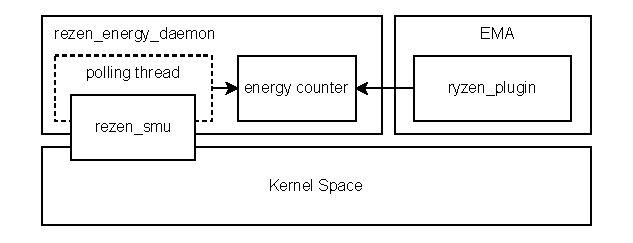
\includegraphics[width=0.7\textwidth]{assets/methodology_improved_concept}
    \caption{
      Suggested improved concept of the \gls{EMA} Ryzen Plug-in realization.
    }
    \label{fig:method}
\end{figure}

First, to address the accuracy issues related to Ryzen Plug-in readings in
\gls{EMA} a draft concept was developed (see \cref{fig:method}). A dedicated
system daemon process is the core part of this concept which should be
responsible for polling the power readings via the kernel driver, integrate
them (readings) to energy values and update the shared counter, which in
turn can be accessed from user-space in the same fashion as various files in
\texttt{powercap} Linux framework for \gls{RAPL} \footnote{\url{
  https://www.kernel.org/doc/html/latest/power/powercap/powercap.html
}}.

Realization of such method would benefit from higher refresh rates of energy
readings from \gls{PM} Table, thus potentially provide higher accuracy and
precision \cref{sec:find:rates}.

The integration method should also be a target of refinements and
improvements \cref{para:practical}.

The second direction would be revising the realization of \emph{Ryzen Plug-in}
for \gls{EMA}, trying to identify any potential bugs, especially related
to numeric type conversions, and precision loss. The topic of counter
overflow/wraparound handling should also be addressed.
